% Full instructions available at:
% https://github.com/elauksap/focus-beamertheme

\documentclass{beamer}
\usetheme[numbering=none]{focus}
\usepackage[utf8x]{inputenc} %So spanish accents will work%
\usepackage{hyperref}
\usepackage{listings}
\usepackage{color}
\usepackage{verbatim}
\usepackage{inconsolata}

\definecolor{codegray}{rgb}{0.5,0.5,0.5}
\definecolor{codecyan}{RGB}{0, 255, 255}
\definecolor{codeyellow}{RGB}{240,219,78}

\lstdefinestyle{mystyle}{
    commentstyle=\color{codeyellow},
    keywordstyle=\color{magenta},
    numberstyle=\color{codegray},
    stringstyle=\color{codecyan},
    basicstyle=\ttfamily\small,
    breakatwhitespace=false,         
    breaklines=true,                 
    captionpos=b,                    
    keepspaces=true,
    showspaces=false,                
    showstringspaces=false,
    showtabs=false,                  
    tabsize=2
}

\lstdefinelanguage{JavaScript}{
keywords={typeof, new, true, false, catch, function, return, null, catch, switch, var, let, if, in, while, do, else, case, break},
ndkeywords={class, export, boolean, throw, implements, import, this},
ndkeywordstyle=\color{darkgray}\bfseries,
sensitive=false,
comment=[l]{//},
morecomment=[s]{/*}{*/},
morestring=[b]',
morestring=[b]",
morestring=[b]`,
}
\lstset{style=mystyle, escapeinside=||}
\title{Javascript}
\subtitle{Hour of Code 2018}

\titlegraphic{
\includegraphics[scale=0.13]{images/js_logo.png}}
\institute{Universidad de Valladolid}
\date{27 Oct 2018}

\begin{document}
\begin{frame}
        \maketitle
\end{frame}
    % PARAGRAPH SPACING. -----------------------------------------------------------------
    \setlength{\parskip}{\baselineskip}%
    \setlength{\parindent}{0pt}%

\begin{frame}{Que es Javascript}
    	\pause
        Javascript (también llamado JS) es un lenguaje de programación originado en 1995.\pause

    	Es conocido principalmente por su uso en desarrollo web, permitiendo que un usuario pueda interaccionar con una pagina web.
\end{frame}
\begin{frame}{Que es Javascript}
        Javascript es un lenguaje... \bigskip
        \begin{itemize}
            \item interpretado\pause
            \item que usa tipado débil\pause
            \item dinámico
    \end{itemize}
\end{frame}
    
\begin{frame}{Javascript es interpretado}
        \pause
        Un lenguaje \textbf{interpretado} es aquel que es traducido a código maquina a medida que se ejecuta, mientras que un lenguaje \textbf{compilado} es aquel que se traduce a código maquina antes de ejecutarse.\pause
        \centering
        
        Javascript es un lenguaje interpretado.
\end{frame}
    
\begin{frame}{Javascript usa tipado débil}
        \pause
        Un lenguaje que usa \textbf{tipado débil} no necesita declarar el tipo de sus variables explicitamente, mientras que un lenguaje que usa \textbf{tipado fuerte} necesita declarar el tipo que va a almacenar una variable de antemano.\pause
        \centering
        
        Javascript utiliza tipado débil.
\end{frame}
    
    
    
\begin{frame}{Javascript es dinámico}
        \pause
        Un lenguaje \textbf{dinámico} comprueba los tipos durante la ejecución del programa, mientras que un lenguaje \textbf{estático} los comprueba antes de la ejecución.\pause
        \centering
        
        Javascript es un lenguaje dinámico.
\end{frame}
\begin{frame}[fragile]{C: Compilado, tipado fuerte y estático}\pause
        \lstinputlisting[language=C++]{code_snippets/example.c}\centering
        
        Este programa ha de ser compilado con un compilador.
\end{frame}

\begin{frame}[fragile]{El mismo ejemplo, con Javascript}\pause
        \lstinputlisting[language=JavaScript]{code_snippets/example.js}\centering
\end{frame}

\begin{frame}{Como ejecutar Javascript}\pause
    Hay varias maneras de ejecutar Javascript. La mas accesible es desde vuestro navegador de preferencia (Firefox, Chrome...)\pause
    
    Abrid las herramientas de desarrollador (F12), y buscad la opción de consola.
    \begin{figure}
        \centering
        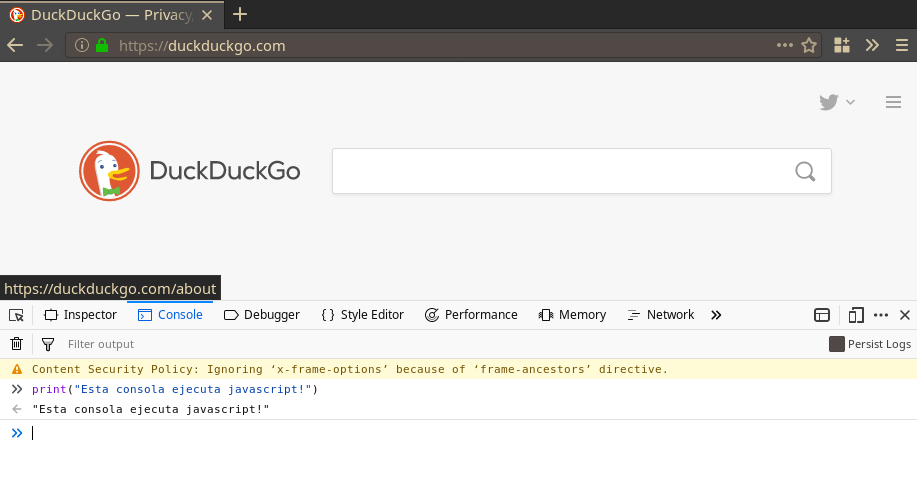
\includegraphics[width=0.75\textwidth]{images/firefox_dev.png}
    \end{figure}
\end{frame}

\begin{frame}{Como ejecutar Javascript}
Para este taller, vamos a utilizar JS Bin, un editor online de Javascript.
    
\centering\url{https://jsbin.com/?js,console}
\end{frame}

\begin{frame}{ECMAScript}
Antes de empezar con Javascript, deberíais saber esto...

ECMAScript es un estándar de lenguajes de programación, y Javascript es una implementación de dicho estándar.

ECMAScript se va actualizando con el tiempo con nuevas funcionalidades, y versiones antiguas de algunos navegadores pueden no estar actualizadas para soportar nuevas versiones de ECMAScript.
\end{frame}

\begin{frame}{ECMAScript}
En este taller, todo lo que os enseñe esta basado en ECMAScript 6 (También llamado ECMAScript 2015, o ES6) y esta soportado por todos los navegadores actuales.

En caso de que tengáis que soportar navegadores antiguos (Internet Explorer 11 y menor, por ejemplo), algunas partes de este taller no funcionaran.
\end{frame}

\begin{frame}{Tipos de datos}
En Javascript, tenemos los siguientes tipos de datos:\bigskip

\begin{columns}[t, onlytextwidth]
            \column{0.5\textwidth}
                \textbf{Primitivos:}
                \begin{itemize}
                    \item Number
                    \item String
                    \item Boolean
                    \item Null
                    \item Undefined
                    \item Symbol
                \end{itemize}
            
            \column{0.5\textwidth}
                \textbf{No primitivos:}
                \begin{itemize}
                    \item Object
                \end{itemize}
        \end{columns}
\end{frame}

\begin{frame}{Numbers}
Un \textbf{number} (Numero) es un tipo de dato numérico.

A diferencia de otros lenguajes, no hay distintos tipos dependiendo de si el numero es decimal o no, o de cuanto espacio se quiera reservar (short, int, long, double, float...)

En Javascript, solo hay un unico tipo, number. Este es similar a un double en otros lenguajes de programacion (64 bits, punto flotante)
\end{frame}

\begin{frame}[fragile]{Numbers}
\begin{lstlisting}[language=JavaScript]
let numero = 42;
typeof(numero); // "number"|\pause|

let comaflotante = 3.141592;
typeof(comaflotante); // "number"|\pause|

// Tambien puedes utilizar notacion cientifica
let notacionExp = 123e5; // 123 * (10^5) = 12300000|\pause|

// O hexadecimal (0x) y octal (0)
let hexadecimalNum = 0xFF; // 255
let octalNum = 0147 // 103
\end{lstlisting}    
\end{frame}

\begin{frame}[fragile]{Numbers: Casos especiales}
\begin{lstlisting}[language=JavaScript]
// Y que pasa si hago esto?
let divisionByZero = 1/0;|\pause| // Infinity|\pause|
let negativeDivisionByZero = -1/0; // -Infinity|\pause|

// Y un numero extremadamente grande?|\pause|
let giganticNumber = 1e9999; // Infinity
let giganticNegativeNumber = -1e9999; // -Infinity

// Infinity e -Infinity son de tipo number!
typeof(Infinity); // "number"
typeof(-Infinity); // "number"

// Y esto de aqui?
let divisionByTomato = 4 / "tomato";|\pause| // "NaN"
\end{lstlisting}    
\end{frame}

\begin{frame}{Numbers: Casos especiales}
NaN es un numero especial. Como habréis notado, Javascript no suele devolver errores ante casos extraños.

Ya entraremos en detalle acerca de como Javascript maneja estos casos, pero por ahora centrémonos en NaN.\pause

NaN (Not a Number; No es un número) es un valor numérico que Javascript devuelve siempre que no encuentre un valor legal en una operacion aritmetica (como una string, con excepciones que ya mencionaremos)
\end{frame}

\begin{frame}[fragile]{Numbers: Operaciones}
\begin{lstlisting}[language=JavaScript]
let num1 = 9, num2 = 3;

// Operador de suma: +
let sumaNums = num1 + num2; // 12

// Operador de resta: -
let restaNums = num1 - num2; // 6

// Operador de producto: *
let productoNums = num1 * num2; // 27

// Operador de division: /
let divisionNums = num1 / num2; // 3

// Operador de resto: %
let restoNums = num1 % num2; // 0
\end{lstlisting}
\end{frame}

\begin{frame}[fragile]{Numbers: Operaciones}
\begin{lstlisting}[language=JavaScript]
// Operador de incremento: ++
num1++; // num1 = 10;

// Operador de decremento: --
num2--; // num2 = 2;
\end{lstlisting}

\begin{block}{Cuidado! Operaciones con NaN}
Cualquier operación que tenga NaN en alguno de sus operandos devolverá NaN. 
\begin{lstlisting}
let someOperation = 46 + (38 % NaN) * 27; // NaN
\end{lstlisting}
\end{block}
\end{frame}

\begin{frame}[fragile]{Numbers: Punto flotante}
Recordad que en Javascript, \textbf{todos} los números son de punto flotante. Esto puede dar lugar a imprecisiones, y debéis de tener cuidado con estas.

\begin{lstlisting}[language=JavaScript]
0.1 + 0.2; // 0.30000000000000004

0.1 + 0.2 == 0.3; // false
\end{lstlisting}
\end{frame}

\begin{frame}[fragile]{Strings}
Un \textbf{String} es una cadena de caracteres usada para representar texto.

Puedes usar single quotes ('), double quotes (") o backticks (`) para delimitar un string, aunque estos últimos son un caso especial que ya mencionaremos.

\begin{lstlisting}[language=JavaScript]
let singleQuotes = 'Soy una cadena de caracteres!';
let doubleQuotes = "Yo tambien!";
let backTicks = `Y yo!`;

typeof(singleQuotes); // "string"
\end{lstlisting}
\end{frame}

\begin{frame}[fragile]{Strings}
En caso de que querais utilizar alguno de los caracteres delimitantes en una string, teneis dos formas de hacerlo:
\begin{itemize}
\item Utilizar un delimitador distinto: 
\begin{lstlisting}[language=JavaScript]
let stringConSingleQuotes = "Uso ' y `!"

let stringConDoubleQuotes = 'Y yo uso " y `!'

let stringConAmbos = `Tengo " y ' sin problemas!`
\end{lstlisting}
\item Escapar el caracter con \textbackslash:
\begin{lstlisting}[language=JavaScript]
let soloUsoDoubles = "Esto \" funciona!"
\end{lstlisting}
\end{itemize}
\end{frame}

\begin{frame}[fragile]{Strings: Concatenación}
Las strings solo tienen un operador: concatenación (+)
\begin{lstlisting}[language=JavaScript]
let nombre = "Alberto";
let apellido = "Gonzalez";

let nombreConApellido = nombre + " " + apellido;
// nombreConApellido = "Alberto Gonzalez"
\end{lstlisting}
\begin{block}{Cuidado! No confundáis los operadores}
Tanto el operador de concatenación como el de adición utilizan el mismo símbolo (+), pero son dos operadores completamente distintos. Ya entraremos en detalle acerca de esto mas adelante.
\end{block}
\end{frame}

\begin{frame}[fragile]{Strings: template strings}
En caso de que quieras tener una string con valores de variables, usar template strings puede ser muy util para facilitar la tarea.

Esto solo funciona si el string usa backticks como delimitador (`)\bigskip

\begin{lstlisting}[language=JavaScript]
let nombre = "Alberto";
let apellido = "Gonzalez";

let nombreConApellido = `${nombre} ${apellido}`;
// nombreConApellido = "Alberto Gonzalez"
\end{lstlisting}
\end{frame}

\begin{frame}[fragile]{Boolean}
Un \textbf{Boolean} (Booleano) es un tipo de dato que solo tiene dos valores: true (verdadero) o false (falso).

\begin{lstlisting}[language=JavaScript]
let verdadero = true;
let falso = false;

typeof(verdadero); // "boolean"
typeof(falso); // "boolean"

\end{lstlisting}
\end{frame}

\begin{frame}[fragile]{Null}
\textbf{Null} es un tipo de dato que solo tiene un valor: Null.

Null se usa para indicar que algo no tiene ningún valor; que esta vacío.

\begin{lstlisting}[language=JavaScript]
let vacio = null;

typeof(vacio); // "object" (por motivos de legacy)

\end{lstlisting}
\end{frame}

\begin{frame}[fragile]{Undefined}
\textbf{Undefined} es un tipo de dato que solo tiene un valor: undefined.

Undefined se usa para indicar que algo no tiene ningun valor asignado.

\begin{lstlisting}[language=JavaScript]
let indefinido;

typeof(indefinido); // "undefined"
\end{lstlisting}
\end{frame}

\begin{frame}{Diferencia entre null y undefined}
null y undefined son dos cosas distintas, pese a parecer identicas. Aqui teneis un ejemplo visual.

    \begin{figure}
        \centering
        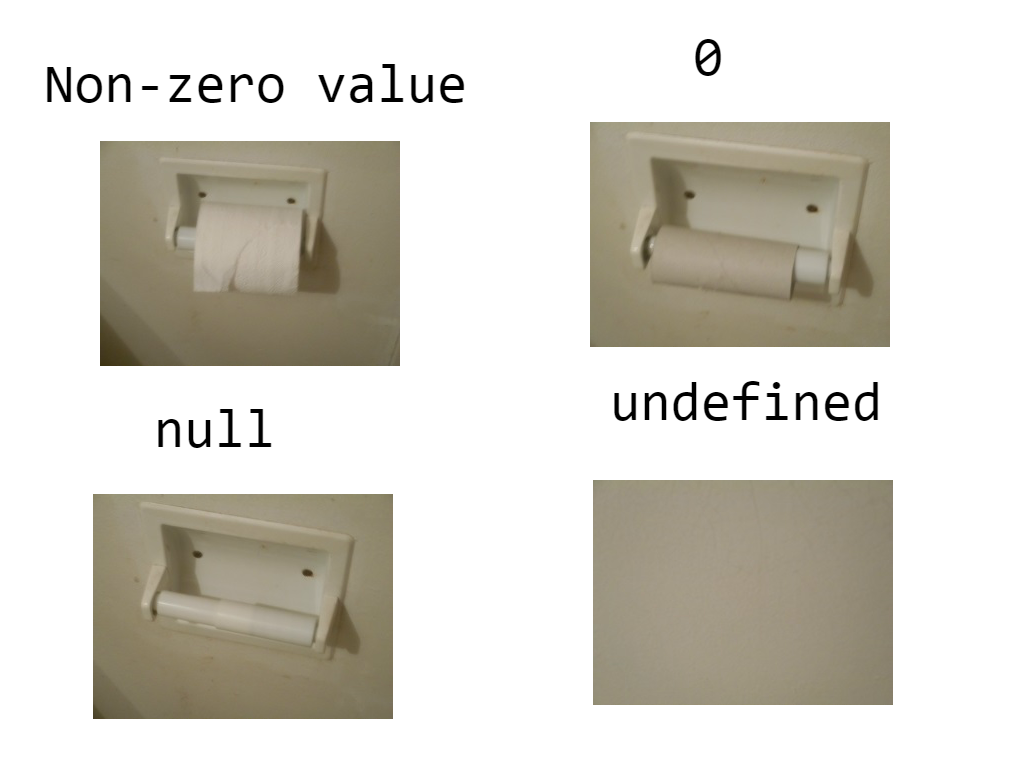
\includegraphics[width=0.7\textwidth]{images/undefinednull.png}
    \end{figure}
\end{frame}

\begin{frame}{Diferencia entre null y undefined}
\begin{itemize}
    \item Undefined indica que algo simplemente no esta ahi, y es el valor que toma cualquier variable por defecto.
    \item Null indica explicitamente que el valor de algo es nulo, y has de asignarlo explicitamente a algo.
\end{itemize}
\end{frame}
\end{document}
